% After Change 1: "Upload File Checks" and "Upload Widget Choice" (both modified)
\documentclass[border=8pt]{standalone}
\usepackage{tikz}
% Shared look for all diagrams. Grey = Django class, blue = app class, green = added in Part 2.
\usetikzlibrary{positioning,shapes.multipart,arrows.meta,fit,backgrounds}
\definecolor{djangoC}{HTML}{E6E6E6}
\definecolor{appC}{HTML}{D6E8FA}
\definecolor{newC}{HTML}{D5F0D5}
\newcommand{\role}[1]{{\footnotesize\itshape #1}}
\tikzset{
  box/.style={draw, rectangle split, rectangle split parts=2, align=center,
              font=\small, inner sep=5pt, minimum width=3.6cm},
  djcls/.style={box, rectangle split part fill={djangoC,white}},
  appcls/.style={box, rectangle split part fill={appC,white}},
  newcls/.style={box, rectangle split part fill={newC,white}},
  plain/.style={draw, align=center, font=\small, inner sep=5pt, minimum width=3.2cm, minimum height=1cm},
  note/.style={draw, align=left, font=\footnotesize, fill=yellow!12, inner sep=4pt},
  inherits/.style={-{Triangle[open,length=3mm,width=3mm]}, thick},
  uses/.style={-{Stealth[length=2.5mm]}, thick},
  lbl/.style={font=\footnotesize, fill=white, inner sep=1.5pt},
  num/.style={circle, draw, fill=white, font=\scriptsize\bfseries, inner sep=1.2pt},
}

\begin{document}
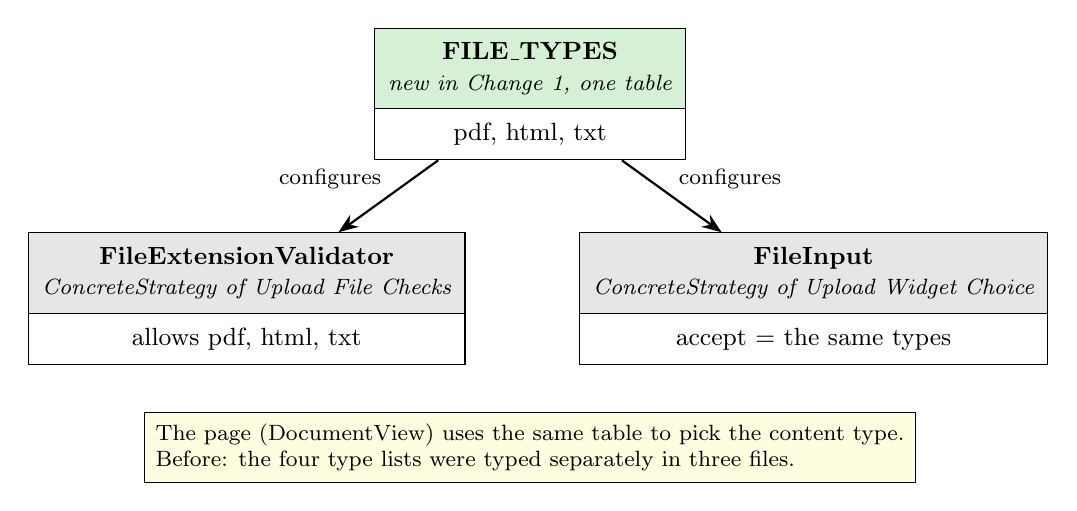
\begin{tikzpicture}
\node[newcls] (ft) at (0,0) {\textbf{FILE\_TYPES} \\ \role{new in Change 1, one table}
  \nodepart{second} pdf, html, txt};
\node[djcls] (fev) at (-3.6,-2.6) {\textbf{FileExtensionValidator} \\ \role{ConcreteStrategy of Upload File Checks}
  \nodepart{second} allows pdf, html, txt};
\node[djcls] (fi) at (3.6,-2.6) {\textbf{FileInput} \\ \role{ConcreteStrategy of Upload Widget Choice}
  \nodepart{second} accept = the same types};
\draw[uses] (ft) -- node[lbl, above left=1pt] {configures} (fev);
\draw[uses] (ft) -- node[lbl, above right=1pt] {configures} (fi);
\node[note, below=0.5cm of ft, yshift=-2.7cm] {The page (DocumentView) uses the same table to pick the content type.\\ Before: the four type lists were typed separately in three files.};
\end{tikzpicture}
\end{document}
